% This must be in the first 5 lines to tell arXiv to use pdfLaTeX, which is strongly recommended.


\pdfoutput=1
% In particular, the hyperref package requires pdfLaTeX in order to break URLs across lines.

\documentclass[11pt]{article}

% Change "review" to "final" to generate the final (sometimes called camera-ready) version.
% Change to "preprint" to generate a non-anonymous version with page numbers.
\usepackage[final]{acl}

% Standard package includes
\usepackage{times}
\usepackage{latexsym}

% For proper rendering and hyphenation of words containing Latin characters (including in bib files)
\usepackage[T1]{fontenc}
% For Vietnamese characters
% \usepackage[T5]{fontenc}
% See https://www.latex-project.org/help/documentation/encguide.pdf for other character sets

% This assumes your files are encoded as UTF8
\usepackage[utf8]{inputenc}

% This is not strictly necessary, and may be commented out,
% but it will improve the layout of the manuscript,
% and will typically save some space.
\usepackage{microtype}

% This is also not strictly necessary, and may be commented out.
% However, it will improve the aesthetics of text in
% the typewriter font.
\usepackage{inconsolata}

%Including images in your LaTeX document requires adding
%additional package(s)
\usepackage{graphicx}

\usepackage{multirow}

% If the title and author information does not fit in the area allocated, uncomment the following
%
%\setlength\titlebox{<dim>}
%
% and set <dim> to something 5cm or larger.

% \title{Instructions for *ACL Proceedings}

\title{Chinchunmei at SemEval-2025 Task 11: Boosting the Large Language Model's Capability of Emotion Perception using Contrastive Learning}

\author{
  Tian Li\textsuperscript{1},
  Yujian Sun\textsuperscript{2},
  Huizhi Liang\textsuperscript{1}
\\
  \textsuperscript{1}School of Computing, Newcastle University, Newcastle upon Tyne, UK\\
  \textsuperscript{2}Shumei AI Research Institute, Beijing, China
\\
  \texttt{t.li56@newcastle.ac.uk}, \texttt{sunyujian@ishumei.com},\\\texttt{huizhi.liang@newcastle.ac.uk}
}

% Author information can be set in various styles:
% For several authors from the same institution:
% \author{Author 1 \and ... \and Author n \\
%         Address line \\ ... \\ Address line}
% if the names do not fit well on one line use
%         Author 1 \\ {\bf Author 2} \\ ... \\ {\bf Author n} \\
% For authors from different institutions:
% \author{Author 1 \\ Address line \\  ... \\ Address line
%         \And  ... \And
%         Author n \\ Address line \\ ... \\ Address line}
% To start a separate ``row'' of authors use \AND, as in
% \author{Author 1 \\ Address line \\  ... \\ Address line
%         \AND
%         Author 2 \\ Address line \\ ... \\ Address line \And
%         Author 3 \\ Address line \\ ... \\ Address line}

%\author{First Author \\
%  Affiliation / Address line 1 \\
%  Affiliation / Address line 2 \\
%  Affiliation / Address line 3 \\
%  \texttt{email@domain} \\\And
%  Second Author \\
%  Affiliation / Address line 1 \\
%  Affiliation / Address line 2 \\
%  Affiliation / Address line 3 \\
%  \texttt{email@domain} \\}

%\author{
%  \textbf{First Author\textsuperscript{1}},
%  \textbf{Second Author\textsuperscript{1,2}},
%  \textbf{Third T. Author\textsuperscript{1}},
%  \textbf{Fourth Author\textsuperscript{1}},
%\\
%  \textbf{Fifth Author\textsuperscript{1,2}},
%  \textbf{Sixth Author\textsuperscript{1}},
%  \textbf{Seventh Author\textsuperscript{1}},
%  \textbf{Eighth Author \textsuperscript{1,2,3,4}},
%\\
%  \textbf{Ninth Author\textsuperscript{1}},
%  \textbf{Tenth Author\textsuperscript{1}},
%  \textbf{Eleventh E. Author\textsuperscript{1,2,3,4,5}},
%  \textbf{Twelfth Author\textsuperscript{1}},
%\\
%  \textbf{Thirteenth Author\textsuperscript{3}},
%  \textbf{Fourteenth F. Author\textsuperscript{2,4}},
%  \textbf{Fifteenth Author\textsuperscript{1}},
%  \textbf{Sixteenth Author\textsuperscript{1}},
%\\
%  \textbf{Seventeenth S. Author\textsuperscript{4,5}},
%  \textbf{Eighteenth Author\textsuperscript{3,4}},
%  \textbf{Nineteenth N. Author\textsuperscript{2,5}},
%  \textbf{Twentieth Author\textsuperscript{1}}
%\\
%\\
%  \textsuperscript{1}Affiliation 1,
%  \textsuperscript{2}Affiliation 2,
%  \textsuperscript{3}Affiliation 3,
%  \textsuperscript{4}Affiliation 4,
%  \textsuperscript{5}Affiliation 5
%\\
%  \small{
%    \textbf{Correspondence:} \href{mailto:email@domain}{email@domain}
%  }
%}

\begin{document}
\maketitle
\begin{abstract}
\iffalse
This document is a supplement to the general instructions for *ACL authors. It contains instructions for using the \LaTeX{} style files for ACL conferences.
The document itself conforms to its own specifications, and is therefore an example of what your manuscript should look like.
These instructions should be used both for papers submitted for review and for final versions of accepted papers.
\fi
% 在text-based emotion detection领域,如何处理由表达与背景多样化所带来的识别挑战一直是热门研究课题。本次SemEVAL-2025 task11 提出了“Bridging the Gap in Text-Based Emotion Detection” 挑战比赛,包含多标签分类(track a)和情感程度预测(track b)两个赛题。两个赛题的情感标签为anger, fear, joy, sadness, surprise 与disgust,并且包含多达33个不同的语言样本。在本次参赛中,我们基于对比的思想,详细探索了基于样本对比(Contrastive Reasoning Calibration)和基于生成对比 (DPO,SimPO)的两种思路在情感识别上的收益。基于样本对比方案为训练模型通过比较两条样本从而生成更靠谱的预测。基于生成对比的方案为训练模型区分正确的预测与错误的预测从而生成更好的预测。所有模型均通过微调LLaMa3-instruct-8B 得到。最终我们的系统在tracka和trackb的英语语种上分别取得了第12和第七的排名,同时在其他语种上名列前茅。

% Handling the challenges posed by expression and background diversity in text-based emotion detection has long been a key research topic. To advance the exploration of these challenges, the SemEval-2025 Task 11, “Bridging the Gap in Text-Based Emotion Detection”, presents a competition with two sub-tasks: multi-label classification (Track A) and emotion intensity prediction (Track B). Both tracks cover six emotion labels—anger, fear, joy, sadness, surprise, and disgust—and include samples from 28 different languages.

The SemEval-2025 Task 11, Bridging the Gap in Text-Based Emotion Detection, introduces an emotion recognition challenge spanning over 28 languages. This competition encourages researchers to explore more advanced approaches to address the challenges posed by the diversity of emotional expressions and background variations. It features two tracks: multi-label classification (Track A) and emotion intensity prediction (Track B), covering six emotion categories: anger, fear, joy, sadness, surprise, and disgust.
In our work, we systematically explore the benefits of two contrastive learning approaches: sample-based (Contrastive Reasoning Calibration) and generation-based (DPO, SimPO) contrastive learning. The sample-based contrastive approach trains the model by comparing two samples to generate more reliable predictions. The generation-based contrastive approach trains the model to differentiate between correct and incorrect generations, refining its prediction. All models are fine-tuned from LLaMa3-Instruct-8B. Our system achieves 12th place in Track A and 7th place in Track B for English, while ranking among the top-tier performing systems for other languages.

\end{abstract}

\section{Introduction}
\iffalse
These instructions are for authors submitting papers to *ACL conferences using \LaTeX. They are not self-contained. All authors must follow the general instructions for *ACL proceedings,\footnote{\url{http://acl-org.github.io/ACLPUB/formatting.html}} and this document contains additional instructions for the \LaTeX{} style files.

The templates include the \LaTeX{} source of this document (\texttt{acl\_latex.tex}),
the \LaTeX{} style file used to format it (\texttt{acl.sty}),
an ACL bibliography style (\texttt{acl\_natbib.bst}),
an example bibliography (\texttt{custom.bib}),
and the bibliography for the ACL Anthology (\texttt{anthology.bib}).
\fi

% Text-based Emotion Detection(TBED)一直都是NLP研究中的一个热点。其已被广泛应用于社交媒体分析,心理疾病治疗,用户喜好预测,以及对话系统。基于对Emotion的定义的差异,TBED可简单分为两类做法:(1).若情绪被划分为不同的类别,则情绪识别则主要采用分类算法,通过模型预测文本是否包含对应的情绪 (2). 若情绪被定义为为相互关联的实体且每个实体存在强度差异,则情绪识别大多采用回归算法,通过预测文本在多个情绪维度上的强度来达成目标。同时,由于情绪表达非常敏感且复杂,情绪识别还面临以下挑战:1. 不同情绪的差异往往非常细微,且情绪的表达也往往通过隐形的方式(比喻,或引发情绪的情况)表达出来。 2. 不同的文化背景与语言也会影响情绪的判断。这些挑战暗示了情绪识别不能仅依赖特定字典进行判断,而是需要结合文化,语种,背景知识,与更加先进的语义理解来给出综合判断。

Text-Based Emotion Detection (TBED) has long been a prominent research area in NLP, with widespread applications in social media analysis \cite{kuamri2017real, salam2018emotion, cassab2020ontology}, mental health treatment \cite{kusal2021ai, krommyda2021experimental}, and dialogue systems \cite{liu2022dialogueein,ide2022building,hu2021dialoguecrn}. Depending on how emotions are defined, TBED can be broadly categorized into two approaches: (1) Classification-based methods, where emotions are categorized into discrete labels \cite{ekman1969repertoire,plutchik1982psycho}. (2) Scoring-based methods, where emotions are treated as interrelated entities with varying intensity levels \cite{russell1977evidence}. 

However, due to the nuanced and complex nature of emotional expression, TBED faces several key challenges \cite{al2024challenges}: (1) The distinction between different emotions is often subtle, and emotions are often conveyed implicitly—through metaphors or situational cues rather than explicit words. (2) Cultural and linguistic differences influence emotion perception. These challenges make TBED difficult to rely solely on predefined lexicons. A robust TBED system must integrate cultural context, linguistic diversity, background knowledge, and advanced semantic understanding.

% 本次SemEVAL 2025,主办方在TASK11 上提出了 “[**Bridging the Gap in Text-Based Emotion Detection**](https://github.com/emotion-analysis-project/SemEval2025-task11)” 挑战比赛。其比赛数据集包含多达33个不同的语言,且放出了类别标签和强度标签作为赛题A和赛题B。其需识别的情感为“给定一句话读者认为说话者可能感受到什么样的情绪”,而非读者的情感或语句中提到的其他人的情感。其情感类别定义采用了 Ekman’s的框架(Ekman and Friesen, 1981),包含六个基础情感分类: anger,fear, sadness, joy, disgust and surprise。同时其在赛题B的强度预测上,为每个情感设立了4个强度level。其赛题设计既覆盖了现有两大TBED做法,也包含了多语言与细微差异识别的挑战。

SemEval-2025, Task 11, titled "Bridging the Gap in Text-Based Emotion Detection", introduces a multilingual benchmark covering 28 languages\cite{muhammad-etal-2025-semeval,muhammad2025brighterbridginggaphumanannotated,belay-etal-2025-evaluating}. The competition consists of Track A (multi-label classification) and Track B (intensity prediction). The goal is to identify the speaker's perceived emotion in a given sentence. Emotion categories follow Ekman's framework\cite{ekman1969repertoire}, encompassing six basic emotions: anger, fear, sadness, joy, disgust, and surprise. Task B further introduces four intensity levels for each emotion. This competition setup encapsulates both primary TBED methodologies while incorporating challenges in multilingual and fine-grained emotion recognition. 

% 为了兼顾赛题A与赛题B两个任务,同时支持对多达33种语言的情感预测,我们放弃了传统的Encoder分类框架,转而使用了生成式大语言模型。通过监督学习,可以让模型直接生成预测标签,并且不同track 可以使用不同的prompt 模版统一到一个模型中。同时,得益于其预训练预料的规模与语种覆盖率,使用大语言模型也能为多语种情感识别提供良好的支持。

To participate in both tracks and support all languages predictions, we adopt the generative large language model (LLM). This decision is driven by its robust multi-task integration capabilities and strong support for cross-linguistic applications.

\begin{figure*}[h]
% \small
  \centering
  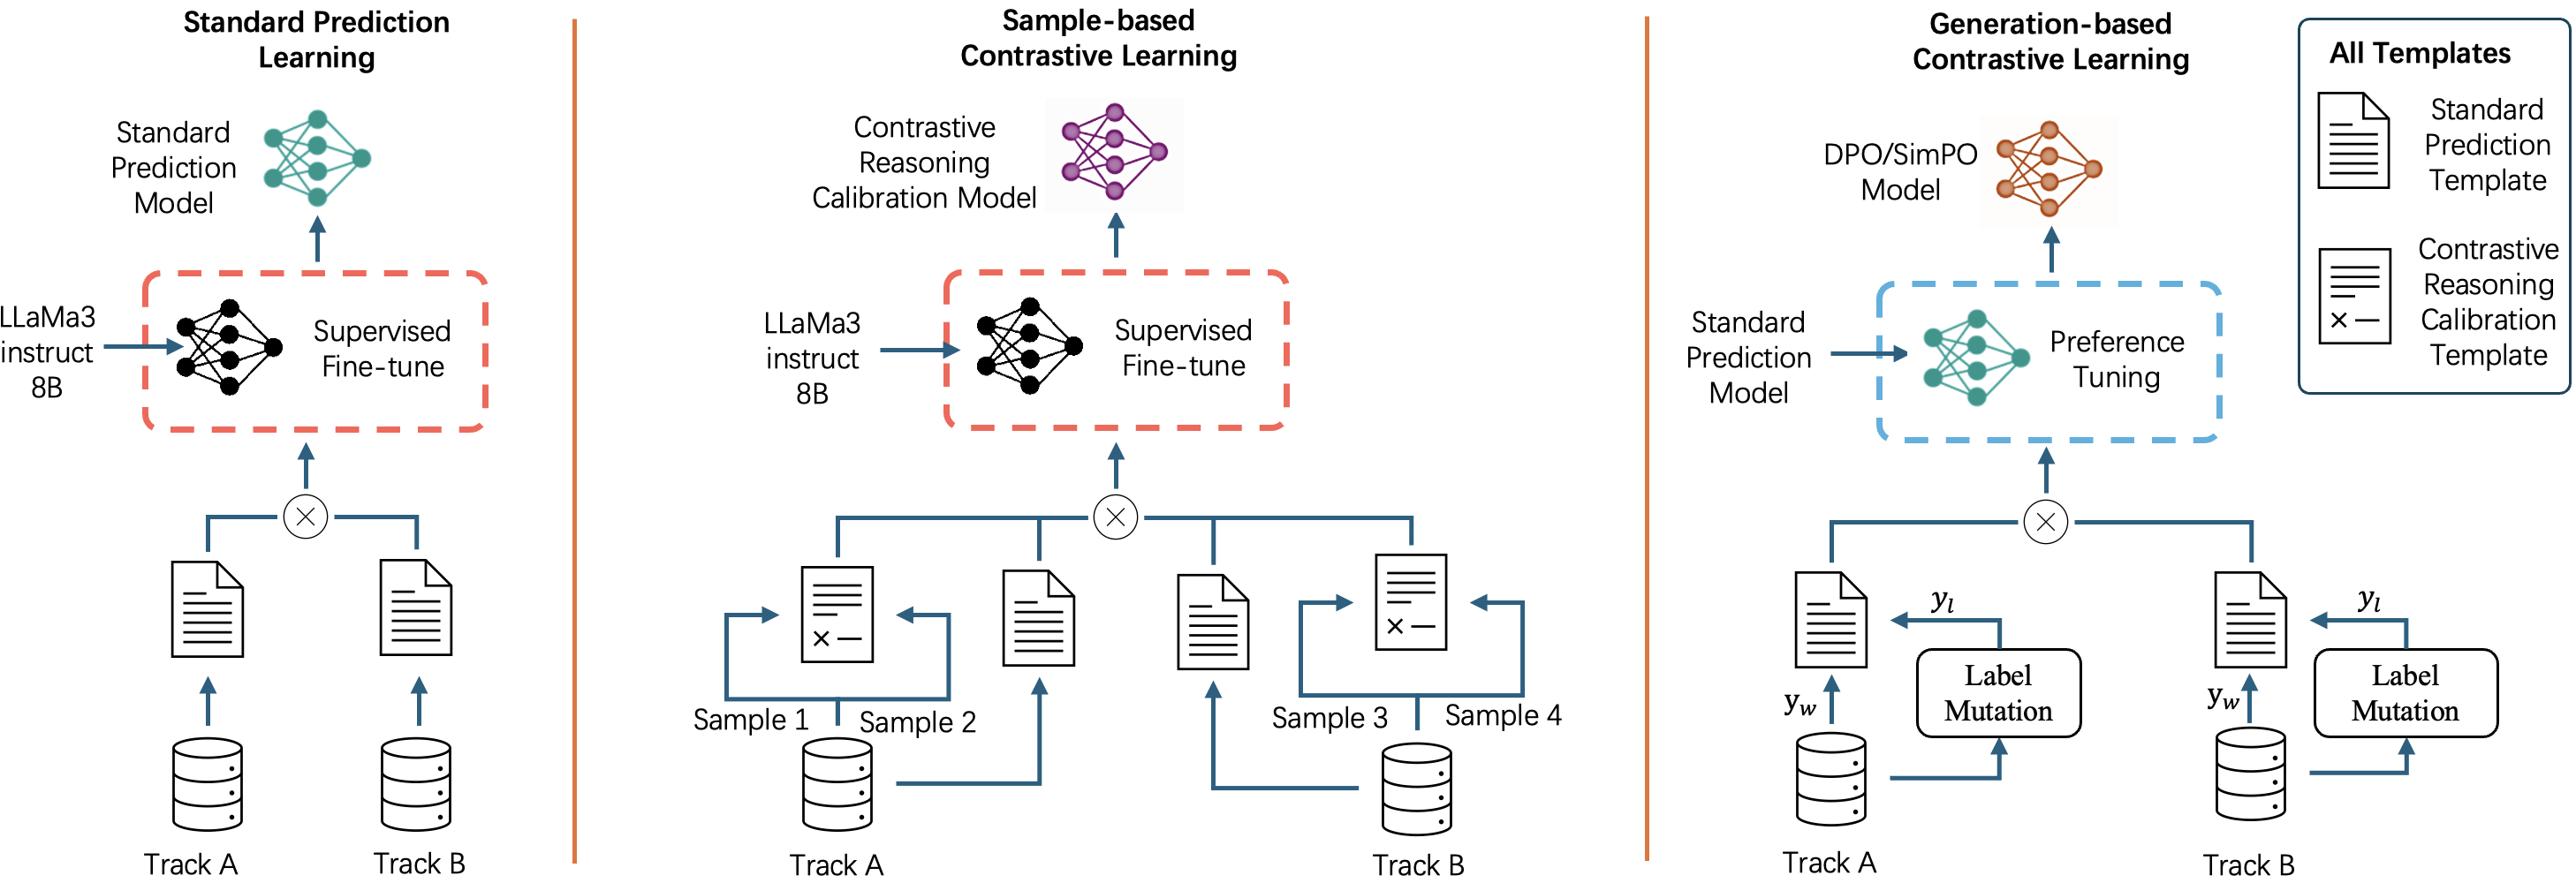
\includegraphics[width=430pt]{Overall}
  \vspace{-5pt}
  \caption{The 3 types of technical solutions we adopted in this competition. On the left is the Standard Prediction training. The middle is the sample-based contrastive training, where Samples 1, 2, 3, and 4 are randomly drawn from the training dataset. On the right is the generation-based contrastive training, where incorrect generations are derived through label mutation.}
  \label{fig:Overall}
 \vspace{-15pt}
\end{figure*}

% 由于情感表达的复杂性和情感标签的不确定性,我们决定采用两套备选方案:基于样本的对比方案和基于生成结果的对比方案。基于样本的对比方案采用CRC技术。其原理是通过样本比较的方式,让模型生成多条更加可靠的的预测并进行投票表决。基于生成结果的对比方案采用偏好优化技术,通过增加正确输出的对数概率并减少错误输出的对数概率,优化模型对于标签的理解能力。受限于计算资源限制,我们探索了DPO与Orpo这两个无需reward model的方案。

In this paper, we explore two alternative types of approaches - sample-based contrastive learning and generation-based contrastive learning - to address the complexity of emotional expression and the ambiguity of sentiment labels. The sample-based approach leverages Contrastive Reasoning Calibration technology (CRC) \cite{li2024chinchunmei}, which enhances prediction reliability by generating multiple predictions through sample comparisons and aggregating them via majority voting. The generation-based approaches employ preference optimization techniques \cite{rafailov2023direct, hong2024orpo, meng2025simpo}, refining the model’s comprehension of sentiment labels by increasing the log probability of correct outputs while reducing that of incorrect ones. Given computational constraints, we only explore DPO \cite{rafailov2023direct} and SimPO\cite{meng2025simpo}, two widely acknowledged methods that do not require the reward model.

% 我们的核心贡献如下

% 1. 我们在有限的计算资源中探索了非英语数据对于英语预测的贡献。令人意外的是,试验结果显示非英语数据的引入会损害英语情感预测的效果,不论是分类任务(track a)还是打分任务(track b).
% 2. 我们详细探索了两种对比方案在该数据集上的效果。在样本对比方案类别上,CRC技术对于该数据集只有负收益。在偏好优化上,也只有DPO在track b上展现了明显的正向收益。SimPO与Orpo不仅会带来效果下降,甚至会让模型丧失规范输出的能力,从而影响结果提取。
% 3. 在最后的比赛排名上,track A与track B的英语语种上我们分别拿到了12/91 和7/42 的成绩。同时在trackA上我们的方案在AMH语种上拿到了第一,16个语种排名前10.在track B上我们的方案在所有的语种排名均在前10.

Our key contributions are as follows:

\begin{itemize}
	\item We explored the impact of non-English data on English sentiment prediction under limited computational resources. Surprisingly, experimental results indicate that incorporating non-English data degrades performance in both classification tasks (Track A) and scoring tasks (Track B).
	\item We conducted an comprehensive evaluation and bad case analysis of two contrastive approaches on the competition dataset. In the sample-based contrastive Learning, CRC technology yielded limited benefit. In the generation-based contrastive Learning, DPO demonstrated a significant positive effect on Track B. Although SimPO has achieved gains on some labels, the overall effect has dropped significantly. 
	\item In the leaderboard, our approach achieved Track A top 10 in 16 languages and 12th in English; Track B top 10 across all languages and 7th in English.
\end{itemize}

\section{Methodology}

% 我们将Track A和Track B都都融合到了一个模型中来节省工作量。通过使用不同的prompt 模版,模型能够按需执行对应的赛题预测。我们首先设计了标准预测任务作为baseline。该任务训练模型直接输出所有标签结果。 其次我们设计了基于样本的对比学习任务。该任务训练模型对比两条样本从而生成更可靠的预测结果。最后我们设计了基于生成的对比学习任务。该任务训练模型区分正确与错误的标签预测输出,使得模型预测更准确。三个任务如图1所示。

To reduce our workload, we integrate both Track A and Track B into the same model by using different prompt templates for each. This unified approach enables the model to dynamically switch between prediction tasks as needed. 

In our explorations, we designed three distinct tasks:
\begin{itemize}
	\item Standard Prediction (Baseline): The model is trained to directly output all emotion labels based on the input text.
	\item Sample-Based Contrastive Learning: The model learns to compare two samples to generate more reliable predictions, leveraging contrastive reasoning to refine label predictions.
	\item Generation-Based Contrastive Learning: The model learns to differentiate between correct and incorrect predictions, improving its ability to generate accurate label outputs.
\end{itemize}

Figure~\ref{fig:Overall} illustrates the training workflow of these three tasks.

\subsection{Standard prediction}
\label{sec:SP}

% 标准任务为利用大语言模型直接进行预测。我们将文本内容整合到预先设计好的prompt模版中作为输入,并将标签结果format成自然语言作为输出的ground truth。通过对格式化好的输入与ground truth进行监督微调得到标准预测的模型。在推理时采用同样的prompt模版整合代推理文字作为输入,通过解析输出的自然语言,拿到各个标签对应的结果。其模版如Appendix 1所示
During sample preparation, we integrate the text content into a pre-designed prompt template as input and format the label results as the ground truth output. The template details can be found in Appendix~\ref{sec:app_PT}. The model is then trained through supervised fine-tune (SFT) using this formatted input and corresponding output.

During inference, we apply the same prompt template to incorporate the input text for prediction. By parsing the generated output, we extract the corresponding label predictions.

\subsection{Sample-based contrastive learning}
\label{sec:CRC}
% CRC任务为样本对比任务。通过训练模型对比两条样本在打分上的异同,从而强化模型对于情感表达细微差异的识别能力。其分为训练和预测两个部分。
In this category, we use CRC, a technique designed to enhance the model’s ability to discern subtle differences in samples. 
% By comparing the scoring variations between two samples, model generated calibrated prediction. 
By having the model compare the score variations between two samples, model can better understand their distinctions and generate calibrated predictions.
% This process consists of training and inference phases.
The key to this task lies in sample preparation and inference process

% 在训练中,我们随机从训练集中抽取两条样本,基于Appendix 2所示的模版构成对比组输入。其目标生成包含两个部分:对比结论与各自预测结果。其对比结论为一段自然语言,总结了两条样本在某个标签上的高低/强弱情况。其预测结果为每个样本在某一标签上的具体打分。其输出模版如Appendix3 所示。

During sample preparation, we randomly select two samples from the training set (Figure~\ref{fig:Overall} middle) and construct a contrastive pair using the template in Appendix~\ref{sec:app_PT}. The target output comprises two components: a contrastive summary and two samples' predictions. The contrastive summary, expressed in natural language, highlights the existence or intensity difference between two samples on a specific label. The predictions provide explicit scores for both samples on the given label. 

% 由于两两随机采样能生成巨量的训练样本,因此我们为track a和track b分别设置了一个样本总数上线。对于track a,每个标签采样3000条对比样本。对于track b,每个标签采样6000条对比样本。这是因为相比于track a ,track b的预测打分多于track a。

Given that random pairwise sampling can generate a vast amount of training data, we imposed an upper limit on the total number of sampled pairs for each track. Specifically, for Track A, we sampled 3,000 contrastive pairs per label, while for Track B, we sampled 6,000 pairs per label, as Track B involves more fine-grained scoring labels compared to Track A.

% 在推理时,每条待预测的样本将同随机抽取的训练样本构建对比组。由于模型对于训练样本预测极为准确,因此我们希望其可作为预测的对比量纲,从而削减预测的不确定性。两条样本被整合到Appendix 2 所示的模版中作为输入,待预测的样本将会被随机放置在位置1或位置2.重复上述过程N次获得N条输入,并由模型生成N条预测结果。最终通过投票机制,将得票最高的打分作为最终输出。

During inference, each test sample is paired with a randomly selected training sample to form a contrastive input. Since the model achieves highly accurate predictions on training samples, these trained samples serve as reliable reference points, reducing prediction uncertainty. The two samples are integrated into the CRC prompt template, with the test sample randomly assigned to either position 1 or position 2. This process is repeated $N$ times to generate $N$ different input instances, producing $N$ predictions. The final score is determined through a voting mechanism, where the most frequently predicted score is selected as the final output.

\subsection{Generation-based contrastive learning}

% 为了强化模型对于打分的敏感性,我们还引入了perference optimiztion。 但是,受限于计算资源,我们仅试验了无需reward model的技术方案。其中包括DPO, SimPO, 以及Orpo

To enhance the model’s sensitivity to scoring, we incorporate preference optimization. However, due to computational constraints, we only explore techniques that do not require a reward model, such as DPO and SimPO.

% Direct Preference Optimization (DPO)通过**相对概率比**来优化语言模型,使其更倾向于偏好回答。(EQ1)。 pai_theta与pai_ref分别指代待优化的模型和初始模型。y_w和y_l分别指代正确的输出和错误的输出。Beta为缩放超参数。该优化流程被用在SFT之后

DPO optimizes the language model by maximizing the relative probability ratio to favor preferred outputs (Eq~\ref{eq:dpo}). Here, $\pi_{\theta}$ and $\pi_{ref}$ represent the target and reference models, respectively, while $y_w$ and $y_l$ denote the correct and incorrect outputs. $\beta$ is a scaling hyperparameter. This optimization process is applied after SFT.

\begin{equation}
\label{eq:dpo}
% \mathcal{L}_{DPO} = \\
-log\sigma(\beta log \frac{\pi_{\theta}(y_w|x)}{\pi_{ref}(y_w|x)} - \beta log \frac{\pi_{\theta}(y_l|x)}{\pi_{ref}(y_l|x)} )
\end{equation}

% SimPO采用类似的优化目标(EQ2)。通过直接优化目标模型的输出概率,SimPO使模型更偏向于偏好答案。然而其简化了DPO,丢弃了参考模型,并且使用生成长度约束loss。该优化流程被用在SFT之后。

SimPO adopts a similar optimization objective (Eq~\ref{eq:simpo}), directly enhancing the probability of the target model’s preferred outputs. However, it simplifies DPO by discarding the reference model and using sequence length to normalize the loss. Additionally, it adopts a hyperparameter $\gamma$ to ensure that the likelihood for the correct response exceeds the incorrect response by $\gamma$. Like DPO, SimPO is also applied after SFT.

\begin{equation}
\label{eq:simpo}
-log\sigma (\frac{\beta}{|y_w|}log\pi_{\theta} (y_w|x) - \frac{\beta}{|y_l|}log\pi_{\theta} (y_l|x) - \gamma)
\end{equation}
\iffalse
% Orpo则是对将对比的思路放到了SFT阶段(EQ3)。通过在SFT loss上新增正负例的对比term,使得高奖励的回答在训练过程中获得更高的学习权重。该流程会直接替换SFT流程。

ORPO integrates the contrastive approach directly into the SFT phase (EQ3). By adding contrastive terms for $y_w$ and $y_l$ in the SFT loss function, ORPO ensures that correct responses receive greater weight during training. This process replaces the original SFT procedure.

\begin{equation}
\mathcal{L}_{SFT} + \beta log\frac{\pi_{\theta}(y_w|x)}{1-\pi_{\theta}(y_w|x)} - \beta log\frac{\pi_{\theta}(y_l|x)}{1-\pi_{\theta}(y_l|x)}
\end{equation}
\fi

% 在训练样本准备时,为了强化模型对标签打分的敏感程度, 我们仅mute了标签打分。Chosen sample 为原ST的ground truth, Rejected sample为同样的SP模版但是使用了muted过后的分数Mute 一个,两个,三个,四个,五个标签的概率为[63.8%, 26.1%, 8.3%, 1.6%, 0.1%]。当mutation触发时,随机从标签剩余取值中取一个作为错误打分。
 
 During sample preparation, to enhance the model's sensitivity to label scoring, we muted only the label scores to generate $y_l$ (Figure~\ref{fig:Overall} right, the Label Mutation block). The $y_w$ corresponds to the original SP ground truth, while the $y_l$ follows the same SP template but with muted scores. The probabilities of muting one, two, three, four, and five labels are [63.8\%, 26.1\%, 8.3\%, 1.6\%, 0.1\%], respectively. When mutation is triggered, a random value is selected from the remaining label values as the incorrect score.
 
 For Track A, each training sample executes five mutations, generating five contrastive samples for generation-based learning. For Track B, mutation is repeated 15 times, creating 15 contrastive samples. These settings ensured that the preference optimization dataset was comparable in size to the CRC dataset, allowing for a fair comparison between sample-based and generation-based approaches.

\section{Experiment}

% Please add the following required packages to your document preamble:
% \usepackage{multirow}
\begin{table*}[]
\centering
\begin{tabular}{llccccccc}
\hline
\multirow{2}{*}{\textbf{Model}} &
  \multirow{2}{*}{\textbf{\begin{tabular}[c]{@{}l@{}}Training\\ Language\end{tabular}}} &
  \multicolumn{7}{c}{\textbf{Track A - eng}} \\
 &
   &
  \textbf{Macro} &
  \textbf{Micro} &
  \textbf{Anger} &
  \textbf{Fear} &
  \textbf{Joy} &
  \textbf{Sadness} &
  \textbf{Surprise} \\ \hline
SP    & English      & \textbf{0.828} & \textbf{0.808} & 0.738          & \textbf{0.876} & 0.824          & 0.818          & 0.784          \\
SP    & Multilingual & 0.820          & 0.802          & 0.742          & 0.865          & 0.814          & 0.808          & 0.780          \\
CRC   & English      & 0.819          & 0.802          & \textbf{0.752} & 0.865          & 0.811          & 0.819          & 0.765          \\
DPO   & English      & 0.827          & 0.806          & 0.736          & 0.875          & 0.816          & 0.821          & \textbf{0.785} \\
SimPO & English      & 0.748          & 0.741          & 0.700          & 0.737          & \textbf{0.827} & \textbf{0.832} & 0.607          \\ \hline
\end{tabular}
\vskip -8pt
\caption{English test results of all models in Track A}
\label{tab:tracka_result}
\vskip -8pt
\end{table*}

% Please add the following required packages to your document preamble:
% \usepackage{multirow}
\begin{table*}[]
\centering
\begin{tabular}{llrrrrrrr}
\hline
\multirow{2}{*}{\textbf{Model}} &
  \multirow{2}{*}{\textbf{\begin{tabular}[c]{@{}l@{}}Training\\ Language\end{tabular}}} &
  \multicolumn{7}{c}{\textbf{Track B - eng}} \\
 &
   &
  \multicolumn{1}{c}{\textbf{Macro}} &
  \multicolumn{1}{c}{\textbf{Micro}} &
  \multicolumn{1}{c}{\textbf{Anger}} &
  \multicolumn{1}{c}{\textbf{Fear}} &
  \multicolumn{1}{c}{\textbf{Joy}} &
  \multicolumn{1}{c}{\textbf{Sadness}} &
  \multicolumn{1}{c}{\textbf{Surprise}} \\ \hline
SP    & English      & 0.845          & 0.823          & \textbf{0.812} & 0.841          & \textbf{0.850} & 0.847          & 0.763          \\
SP    & Multilingual & 0.835          & 0.815          & 0.807          & 0.816          & 0.845          & 0.840          & 0.765          \\
CRC   & English      & 0.828          & 0.805          & 0.796          & 0.807          & 0.836          & 0.837          & 0.750          \\
DPO   & English      & \textbf{0.846} & \textbf{0.824} & 0.810          & \textbf{0.844} & 0.846          & \textbf{0.849} & \textbf{0.773} \\
SimPO & English      & 0.770          & 0.741          & 0.700          & 0.737          & 0.827          & 0.832          & 0.607          \\ \hline
\end{tabular}
\vskip -8pt
\caption{English test set results of all models in Track B}
\label{tab:trackb_result}
\vskip -18pt
\end{table*}

% 本次比赛包含赛题A与赛题B。其中赛题A包含28个语种,赛题B包含11个语种。每个语种包含千计的样本,且部分语种的样本在不同赛题上并不一致。两个赛题的标签为Anger, Fear, Joy, Sadness, Surprise, 和disgust。部分语种存在标签缺失的情况(如英语不包含disgust标签)。待预测内容为不包含前序对话的单句对话文本。赛题A的评估指标为F1 score。赛题B的评估指标为Pearson Correlation。每个赛题包含训练集,开发集与测试集。但是,由于开发集太小,评估指标非常不稳定,因此我们的所有结果均均跑在测试集上。

In this competition, we participate in Track A and Track B. Track A covers 28 languages, while Track B includes 11 languages. Each language contains thousands of samples. Some languages use the same dataset for both Track A and Track B. Both tracks share the same sentiment labels: anger, fear, joy, sadness, surprise, and disgust. However, some languages have missing labels (e.g., English does not include the disgust label). All sample contents are single-turn dialogue without prior dialogue. Track A is evaluated using the F1 score, while Track B uses Pearson Correlation, with both metrics computed in Macro and Micro modes. Macro calculates the overall score across all labels, while Micro first computes per-label scores and then averages them. Although training, development, and test sets are provided, the development set is too small, leading to unstable evaluation results. Therefore, all reported results are based on the test set. Please see Appendix~\ref{sec:app_dev} for the dev set results and discussion.

% 我们所有任务模型均由Llama3-instruct-8B微调而来。这是因为其优异的多语种支持与可接受的计算资源开销。我们利用其tokenizer进行了encoder-decoder流程,通过检查恢复出来的文本与原始文本的一致性来筛选其支持的语种。经过实验,我们确认了该大语言模型支持比赛中的所有语种。

All models in our experiments are fine-tuned from Llama3-Instruct-8B  \cite{dubey2024llama}, selected for its strong multilingual capabilities and acceptable computational cost. To validate its multilingual capabilities in each language, we check the consistency between original and recovered text using its tokenizer to encode and decode the text content. This experiment confirmed that the model supports all competition languages.

% 我们先在标准预测任务上尝试了单英语和多语种的效果以确认多语种对单语言的影响(Section4.1)。 然后我们在英语数据集上分别尝试了CRC,DPO,SimPO等技术,以探索sample-based comparison和generation-based comparison方案对于情感预测任务的收益。CRC模型由ST数据集+CRC数据集通过SFT训练得到。DPO和SimPO模型则是通过对单英语的ST模型进行相应的preference tuning得到。

We first evaluate the impact of multilingual data on English-only performance in the standard prediction (SP) task. Then, we experiment with CRC, DPO, and SimPO on the English dataset to examine the effectiveness of sample-based and generation-based contrastive learning for TBED. The CRC model is trained via SFT on a combination of SP and CRC datasets. DPO and SimPO models are obtained by applying preference tuning to the English-only SP model.

% 我们的所有训练均采用LoRA的方式以节省训练成本。LoRA rank为8,loRA alpha为16,LoRA dropout 为0. 每个任务训练的Epoch 数为3,batch size为128. ST与CRC任务的学习率为4e-4. DPO训练的学习率5e-6,SimPO训练的学习率为1e-6。LR scheduler采用cosine策略,warmup ratio为0.1,batch size为128. 在CRC推理时,Track A的N为3,Track B的N为7。

To reduce training costs, we use LoRA \cite{hu2022lora} for all fine-tuning tasks, with its rank and alpha set as 8 and 16. Each training lasts for 3 epochs with a batch size of 128. Regarding the learning rate (LR), SP and CRC employ 4e-4, DPO adopts 5e-6, and SimPO uses 1e-6. All models are trained using the AdamW optimizer, with $\beta_1=0.8, \beta_2=0.99$. All LR scheduler employs cosine decay with a warmup ratio of 0.1. For CRC inference, we set $N=3$ for Track A and $N=7$ for Track B.

All experiments were conducted using 8-GPU distributed training. Due to limited computational resources, different GPUs were used across various training runs. However, all GPUs were based on the Ada Lovelace or Hopper architecture, allowing us to leverage a wide range of existing acceleration techniques to enhance training efficiency.

\begin{table*}[]
\centering
\begin{tabular}{l|lcc}
\hline
\textbf{ID}                & \multicolumn{1}{c}{\textbf{Text}}           & \textbf{Pred} & \textbf{True} \\ \hline
eng\_test\_track\_a\_02136 &
  \begin{tabular}[c]{@{}l@{}}It was growing harder for him to keep balanced with my \\ legs shifting every few seconds, until finally, I found the \\ right position and his back a good shove with my knee.\end{tabular} &
  0 &
  1 \\
eng\_test\_track\_a\_01815 & So you let it shatter, breaking at my feet. & 1             & 0             \\
eng\_test\_track\_a\_01594 & Dad thought it was just my imagination.     & 0             & 1             \\
eng\_test\_track\_a\_00071 &
  \begin{tabular}[c]{@{}l@{}}There's just something about watching an acne-ridden \\ high school dropout cooking my food that just doesn't \\ sit well in my stomach.\end{tabular} &
  0 &
  1 \\ \hline
\end{tabular}
\vskip -5pt
\caption{Bad cases of the CRC model on the Anger label of Track A}
\label{tab:CRC_badcases}
\vskip -18pt
\end{table*}

\section{Results}

% 表一和表二展示了所有模型在英语测试集上的效果。表一对应track A 多情感标签分类任务,表二对应track B情感程度预测任务。

Tables~\ref{tab:tracka_result} and \ref{tab:trackb_result} present the performance of all models on the English test set. Table 1 corresponds to Track A, the multi-emotion classification task, while Table 2 corresponds to Track B, the emotion intensity prediction task.

\subsection{Multilingual influence}

%不论是track A还是 track B,多语种训练效果都低于单英语训练。这证明了情感的感知在不同语言不同文化背景下存在明显的差异,且这种差异会导致模型对标签的理解存在冲突。关于track a与track b 全语种的 multilingual SP 结果请参见Appendix 5

We observe that multilingual training underperforms compared to English-only training in both Track A and Track B. This finding highlights the significant differences in emotion perception across languages and cultural contexts, which can introduce conflicts in the model’s understanding of sentiment labels. Therefore, we submit the non-English results generated by the multilingual SP model to the leaderboard and discard the multilingual setting in subsequent comparison experiments. For the multilingual SP results of Track A and Track B in all languages, please see Appendix~\ref{sec:app_SP_Multilingual}.

\subsection{Sample-based vs generation-based contrastive learning}

% Table 2 展示了在单英语场景下各个技术方案的最终效果。在track A上,标准预测表现最好。具体到每个标签上,标准预测模型在fear和joy上有超过了其他方案。而在sadness和surprise上,DPO模型效果则以微弱优势取得了第一。在Anger的标签上, CRC模型rank the first。但是在track B上,DPO取得了除Anger标签以外所有评估上的第一名。SimPO效果在所有赛道所有标签上均不达预期。为了进一步分析上述结果背后的原因,我们分析了不同技术的bad case。

In Track A, the SP model performed the best overall. Specifically, it outperformed other approaches on the fear label, while the DPO model achieved a slight advantage on surprise. For anger, the CRC model ranked first, whereas SimPO achieved the best performance on joy and sadness. However, in Track B, DPO secured the top position across all evaluation metrics except for anger and joy. Meanwhile, SimPO lagged significantly behind other systems in both macro and micro performance metrics. To further investigate the underlying reasons for these results, we conducted the bad case analysis for different techniques.

% 在CRC模型上,我们着重分析了track A Anger标签的bad case。我们发现绝大多数错误来自于模型错误判断情感状态为无,占到错误总数的70%。我们随机采样了5条样本并展示在了table3中。可以看到这类样本本身就落在Anger标签定义的boardline上。将其同其他样本进行比对会非常容易导致标签预测反转,进而加大预测的不准确性。这暗示了该数据集先天与sample based comparison 不适配。

For the CRC model, we analyze Track A anger's misclassifications. We find that most misclassifications—accounting for 70\% of the errors—are due to the model incorrectly predicting a neutral emotional state. Table~\ref{tab:CRC_badcases} presents 4 randomly sampled bad cases, illustrating that these instances are on the borderline of the anger definition. Comparing them with other samples can easily influence their predictions, causing uncertainty and error. This suggests that the dataset may not be well-suited for sample-based comparison approach.

% 在DPO模型上,我们着重分析了track B Sadness标签的bad case。 我们发现所有错误同ground truth仅有程度为1的差异。这意味着模型对于标签intensity的感知的敏感性依然存在提升的空间。
For the DPO model, we analyze sadness's wrong cases in Track B. We observed that over 90\% of the errors differed from the ground truth by only one intensity level. This indicates that the model still has room for improvement in its recognition of label intensity.

% 针对SimPO模型,我们发现其效果差的核心原因在于丢失了输出格式,从而导致大量的内容解析错误。该现象揭示了reference 模型对于TBED任务的重要性。尽管其拉大了正确输出与错误输出的概率margin,但其也会导致原先的正确输出不再是概率第一的输出。
Regarding the SimPO model, we figure out that its poor performance primarily stemmed from the loss of output formatting, leading to frequent content parsing errors. This highlights the critical role of the reference model in preference tuning. While SimPO effectively increases the probability margin between correct and incorrect outputs, it may also make correct outputs no longer rank as the top generation.

\section{Conclusion}

% 本次SemEVAL-2025,主办方提出了一份非常具有挑战性的TBED数据集。其包含多标签分类与程度预测,并且包含了超过28个语种。其样本充分展示了情感表达的复杂性,以及不同语言及文化背景所带来的多样性。

The SemEVAL-2025 organizers introduced a highly challenging text-based emotion detection dataset, covering multi-label classification and intensity prediction across 28 languages. The dataset reflects the complexity of emotional expression and the diversity introduced by different linguistic and cultural backgrounds.

% 我们在本次比赛尝试了三类方案。其中baseline方案为标准预测任务。两项改进方案分别为sample based contrastive learning与generation-based contrastive learning。其思想都是通过对比训练的方式强化模型的预测能力,一个对比样本,另一个对比正确与错误的生成。

We explored three types of approaches in this competition. The baseline approach is the standard prediction task. The two enhanced types of approaches were sample-based contrastive learning and generation-based contrastive learning. For the sample-based approach, we try CRC. For the generation-based approach, we explore both DPO and SimPO. They all aim to improve model prediction through contrastive training—one by comparing samples and the other by discriminating between correct and incorrect generations.

% 我们的试验发现,不同语言代表了不同的文化背景,因此multilingual训练并不能为英语emotion detection提供增益。同时由于表达的敏感性,样本对比反而会引入额外的不确定性,从而降低预测的准确性。基于生成的对比学习方案能为程度预测提供稳定的增益,但具体到不同技术上也存在极大的差异。参考模型的约束对于基于生成的对比学习方案极为重要。它能为模型提供稳定的优化基准,防止优化过程过度偏离原始模型分布,从而丧失关键能力(如模版化输出的能力)。

Our experiments reveal that different languages reflect distinct cultural backgrounds, so multilingual training does not improve English emotion detection. Meanwhile, due to the inherent ambiguity of sentiment expressions, sample-based contrastive learning raises additional uncertainty, ultimately reducing prediction accuracy. On the other hand, generation-based contrastive learning provides consistent improvements in intensity prediction, though its effectiveness varies significantly across different techniques. Notably, reference model constraint is crucial in stabilizing generation-based contrastive optimization process. It prevents excessive deviation from the original model distribution, and preserves key capabilities such as structured output generation.

\iffalse
\section{Engines}

To produce a PDF file, pdf\LaTeX{} is strongly recommended (over original \LaTeX{} plus dvips+ps2pdf or dvipdf).
The style file \texttt{acl.sty} can also be used with
lua\LaTeX{} and
Xe\LaTeX{}, which are especially suitable for text in non-Latin scripts.
The file \texttt{acl\_lualatex.tex} in this repository provides
an example of how to use \texttt{acl.sty} with either
lua\LaTeX{} or
Xe\LaTeX{}.

\section{Preamble}

The first line of the file must be
\begin{quote}
\begin{verbatim}
\documentclass[11pt]{article}
\end{verbatim}
\end{quote}

To load the style file in the review version:
\begin{quote}
\begin{verbatim}
\usepackage[review]{acl}
\end{verbatim}
\end{quote}
For the final version, omit the \verb|review| option:
\begin{quote}
\begin{verbatim}
\usepackage{acl}
\end{verbatim}
\end{quote}

To use Times Roman, put the following in the preamble:
\begin{quote}
\begin{verbatim}
\usepackage{times}
\end{verbatim}
\end{quote}
(Alternatives like txfonts or newtx are also acceptable.)

Please see the \LaTeX{} source of this document for comments on other packages that may be useful.

Set the title and author using \verb|\title| and \verb|\author|. Within the author list, format multiple authors using \verb|\and| and \verb|\And| and \verb|\AND|; please see the \LaTeX{} source for examples.

By default, the box containing the title and author names is set to the minimum of 5 cm. If you need more space, include the following in the preamble:
\begin{quote}
\begin{verbatim}
\setlength\titlebox{<dim>}
\end{verbatim}
\end{quote}
where \verb|<dim>| is replaced with a length. Do not set this length smaller than 5 cm.

\section{Document Body}

\subsection{Footnotes}

Footnotes are inserted with the \verb|\footnote| command.\footnote{This is a footnote.}

\subsection{Tables and figures}

See Table~\ref{tab:accents} for an example of a table and its caption.
\textbf{Do not override the default caption sizes.}

\begin{table}
  \centering
  \begin{tabular}{lc}
    \hline
    \textbf{Command} & \textbf{Output} \\
    \hline
    \verb|{\"a}|     & {\"a}           \\
    \verb|{\^e}|     & {\^e}           \\
    \verb|{\`i}|     & {\`i}           \\
    \verb|{\.I}|     & {\.I}           \\
    \verb|{\o}|      & {\o}            \\
    \verb|{\'u}|     & {\'u}           \\
    \verb|{\aa}|     & {\aa}           \\\hline
  \end{tabular}
  \begin{tabular}{lc}
    \hline
    \textbf{Command} & \textbf{Output} \\
    \hline
    \verb|{\c c}|    & {\c c}          \\
    \verb|{\u g}|    & {\u g}          \\
    \verb|{\l}|      & {\l}            \\
    \verb|{\~n}|     & {\~n}           \\
    \verb|{\H o}|    & {\H o}          \\
    \verb|{\v r}|    & {\v r}          \\
    \verb|{\ss}|     & {\ss}           \\
    \hline
  \end{tabular}
  \caption{Example commands for accented characters, to be used in, \emph{e.g.}, Bib\TeX{} entries.}
  \label{tab:accents}
\end{table}

As much as possible, fonts in figures should conform
to the document fonts. See Figure~\ref{fig:experiments} for an example of a figure and its caption.

Using the \verb|graphicx| package graphics files can be included within figure
environment at an appropriate point within the text.
The \verb|graphicx| package supports various optional arguments to control the
appearance of the figure.
You must include it explicitly in the \LaTeX{} preamble (after the
\verb|\documentclass| declaration and before \verb|\begin{document}|) using
\verb|\usepackage{graphicx}|.

\begin{figure}[t]
  \includegraphics[width=\columnwidth]{example-image-golden}
  \caption{A figure with a caption that runs for more than one line.
    Example image is usually available through the \texttt{mwe} package
    without even mentioning it in the preamble.}
  \label{fig:experiments}
\end{figure}

\begin{figure*}[t]
  \includegraphics[width=0.48\linewidth]{example-image-a} \hfill
  \includegraphics[width=0.48\linewidth]{example-image-b}
  \caption {A minimal working example to demonstrate how to place
    two images side-by-side.}
\end{figure*}

\subsection{Hyperlinks}

Users of older versions of \LaTeX{} may encounter the following error during compilation:
\begin{quote}
\verb|\pdfendlink| ended up in different nesting level than \verb|\pdfstartlink|.
\end{quote}
This happens when pdf\LaTeX{} is used and a citation splits across a page boundary. The best way to fix this is to upgrade \LaTeX{} to 2018-12-01 or later.

\subsection{Citations}

\begin{table*}
  \centering
  \begin{tabular}{lll}
    \hline
    \textbf{Output}           & \textbf{natbib command} & \textbf{ACL only command} \\
    \hline
    \citep{Gusfield:97}       & \verb|\citep|           &                           \\
    \citealp{Gusfield:97}     & \verb|\citealp|         &                           \\
    \citet{Gusfield:97}       & \verb|\citet|           &                           \\
    \citeyearpar{Gusfield:97} & \verb|\citeyearpar|     &                           \\
    \citeposs{Gusfield:97}    &                         & \verb|\citeposs|          \\
    \hline
  \end{tabular}
  \caption{\label{citation-guide}
    Citation commands supported by the style file.
    The style is based on the natbib package and supports all natbib citation commands.
    It also supports commands defined in previous ACL style files for compatibility.
  }
\end{table*}

Table~\ref{citation-guide} shows the syntax supported by the style files.
We encourage you to use the natbib styles.
You can use the command \verb|\citet| (cite in text) to get ``author (year)'' citations, like this citation to a paper by \citet{Gusfield:97}.
You can use the command \verb|\citep| (cite in parentheses) to get ``(author, year)'' citations \citep{Gusfield:97}.
You can use the command \verb|\citealp| (alternative cite without parentheses) to get ``author, year'' citations, which is useful for using citations within parentheses (e.g. \citealp{Gusfield:97}).

A possessive citation can be made with the command \verb|\citeposs|.
This is not a standard natbib command, so it is generally not compatible
with other style files.

\subsection{References}

\nocite{Ando2005,andrew2007scalable,rasooli-tetrault-2015}

The \LaTeX{} and Bib\TeX{} style files provided roughly follow the American Psychological Association format.
If your own bib file is named \texttt{custom.bib}, then placing the following before any appendices in your \LaTeX{} file will generate the references section for you:
\begin{quote}
\begin{verbatim}
\bibliography{custom}
\end{verbatim}
\end{quote}

You can obtain the complete ACL Anthology as a Bib\TeX{} file from \url{https://aclweb.org/anthology/anthology.bib.gz}.
To include both the Anthology and your own .bib file, use the following instead of the above.
\begin{quote}
\begin{verbatim}
\bibliography{anthology,custom}
\end{verbatim}
\end{quote}

Please see Section~\ref{sec:bibtex} for information on preparing Bib\TeX{} files.

\subsection{Equations}

An example equation is shown below:
\begin{equation}
  \label{eq:example}
  A = \pi r^2
\end{equation}

Labels for equation numbers, sections, subsections, figures and tables
are all defined with the \verb|\label{label}| command and cross references
to them are made with the \verb|\ref{label}| command.

This an example cross-reference to Equation~\ref{eq:example}.

\subsection{Appendices}

Use \verb|\appendix| before any appendix section to switch the section numbering over to letters. See Appendix~\ref{sec:appendix} for an example.

\section{Bib\TeX{} Files}
\label{sec:bibtex}

Unicode cannot be used in Bib\TeX{} entries, and some ways of typing special characters can disrupt Bib\TeX's alphabetization. The recommended way of typing special characters is shown in Table~\ref{tab:accents}.

Please ensure that Bib\TeX{} records contain DOIs or URLs when possible, and for all the ACL materials that you reference.
Use the \verb|doi| field for DOIs and the \verb|url| field for URLs.
If a Bib\TeX{} entry has a URL or DOI field, the paper title in the references section will appear as a hyperlink to the paper, using the hyperref \LaTeX{} package.

\section*{Limitations}

Since December 2023, a "Limitations" section has been required for all papers submitted to ACL Rolling Review (ARR). This section should be placed at the end of the paper, before the references. The "Limitations" section (along with, optionally, a section for ethical considerations) may be up to one page and will not count toward the final page limit. Note that these files may be used by venues that do not rely on ARR so it is recommended to verify the requirement of a "Limitations" section and other criteria with the venue in question.

\section*{Acknowledgments}

This document has been adapted
by Steven Bethard, Ryan Cotterell and Rui Yan
from the instructions for earlier ACL and NAACL proceedings, including those for
ACL 2019 by Douwe Kiela and Ivan Vuli\'{c},
NAACL 2019 by Stephanie Lukin and Alla Roskovskaya,
ACL 2018 by Shay Cohen, Kevin Gimpel, and Wei Lu,
NAACL 2018 by Margaret Mitchell and Stephanie Lukin,
Bib\TeX{} suggestions for (NA)ACL 2017/2018 from Jason Eisner,
ACL 2017 by Dan Gildea and Min-Yen Kan,
NAACL 2017 by Margaret Mitchell,
ACL 2012 by Maggie Li and Michael White,
ACL 2010 by Jing-Shin Chang and Philipp Koehn,
ACL 2008 by Johanna D. Moore, Simone Teufel, James Allan, and Sadaoki Furui,
ACL 2005 by Hwee Tou Ng and Kemal Oflazer,
ACL 2002 by Eugene Charniak and Dekang Lin,
and earlier ACL and EACL formats written by several people, including
John Chen, Henry S. Thompson and Donald Walker.
Additional elements were taken from the formatting instructions of the \emph{International Joint Conference on Artificial Intelligence} and the \emph{Conference on Computer Vision and Pattern Recognition}.
\fi
% Bibliography entries for the entire Anthology, followed by custom entries
%\bibliography{anthology,custom}
% Custom bibliography entries only
\bibliography{custom}

\appendix

\iffalse
\section{Example Appendix}
\label{sec:appendix}

This is an appendix.

\fi

\section{Appendix}

\subsection{Prompt templates}
\label{sec:app_PT}

Table~\ref{tab:SP_tracka_temp}, \ref{tab:SP_trackb_temp}, \ref{tab:CRC_tracka_temp}, and \ref{tab:CRC_trackb_temp} show the prompt templates used by Standard Prediction and Contrastive Reasoning Calibration on Track A and B, respectively. Preference Tuning also uses the Standard Prediction template.

\begin{table*}[]
\begin{tabular}{l|l}
\hline
\textbf{Input} &
  \textbf{Output} \\ \hline
\begin{tabular}[c]{@{}l@{}}Task Description: \\ You are tasked with determining the perceived emotion(s) of a speaker \\ based on a conversation. Specifically, your goal is to predict the emotions \\ that most people would associate with the speaker's last utterance. The \\ possible emotions are: joy, sadness, fear, anger, surprise, and disgust. The \\ conversation may be in any of the following languages: Afrikaans, \\ Algerian Arabic, Amharic, Emakhuwa, Hausa, Igbo, Kinyarwanda, \\ Moroccan Arabic, Mozambican Portuguese, Nigerian-Pidgin, Oromo, \\ Setswana, Somali, Swahili, Sundanese, Tigrinya, Xitsonga, IsiXhosa, \\ Yoruba, isiZulu Arabic, Chinese, Hindi, Indonesian, Javanese, Marathi \\ English, German, Romanian, Russian, Latin American Spanish, Tatar, \\ Ukrainian, Swedish, Mozambican Portuguese, and Brazilian Portuguese. \\ \\ Instructions: \\ 1. The language of the conversation will be explicitly indicated at the \\ first place. \\ 2. Each turn in the conversation will be marked with "Speaker1" or \\ "Speaker2" to indicate the speaker. \\ 3. You need to predict the emotions based on the last utterance from \\ "Speaker1" (and any additional context or dialogue history if provided). \\ 4. For each emotion, indicate whether it applies using binary labels: 1 \\ (emotion is present) or 0 (emotion is absent). \\ \\ Example Output Format: \\ joy: \{\{ 1 or 0 \}\}, sadness: \{\{ 1 or 0 \}\}, fear: \{\{ 1 or 0 \}\}, anger: \{\{ 1 or \\ 0 \}\}, (optional) surprise: \{\{ 1 or 0 \}\}, (optional) disgust: \{\{ 1 or 0 \}\}. \\ \\ Language: \\ \{lan\}\\ \\ Content: \\ Speaker1: \{text\}\end{tabular} &
  \begin{tabular}[c]{@{}l@{}}joy: \{joy\}, \\ sadness: \{sadness\}, \\ fear: \{fear\}, \\ anger: \{anger\}, \\ surprise: \{surprise\}, \\ disgust: \{disgust\}.\end{tabular} \\ \hline
\end{tabular}
\caption{Standard prediction template for Track A}
\label{tab:SP_tracka_temp}
\end{table*}

\begin{table*}[]
\begin{tabular}{l|l}
\hline
\textbf{Input} &
  \textbf{Output} \\ \hline
\begin{tabular}[c]{@{}l@{}}Task Description: \\ You are tasked with predicting the intensity for each of the perceived \\ emotion classes of a speaker based on a conversation. Specifically, your \\ prediction should represent the emotional intensity most people \\ associate with the speaker's last utterance. The possible emotion classes \\ are: joy, sadness, fear, anger, surprise, and disgust. The conversation may \\ be in any of the following languages: Afrikaans, Algerian Arabic, \\ Amharic, Emakhuwa, Hausa, Igbo, Kinyarwanda, Moroccan Arabic, \\ Mozambican Portuguese, Nigerian-Pidgin, Oromo, Setswana, Somali, \\ Swahili, Sundanese, Tigrinya, Xitsonga, IsiXhosa, Yoruba, isiZulu Arabic, \\ Chinese, Hindi, Indonesian, Javanese, Marathi English, German, \\ Romanian, Russian, Latin American Spanish, Tatar, Ukrainian, Swedish, \\ Mozambican Portuguese, and Brazilian Portuguese. \\ \\ Instructions: \\ 1. The language of the conversation will be explicitly indicated at the first \\ place. \\ 2. Each turn in the conversation will be marked with "Speaker1" or \\ "Speaker2" to indicate the speaker. \\ 3. You need to predict the emotion intensity based on the last utterance \\ from "Speaker1" (and any additional context or dialogue history if \\ provided). \\ 4. For each emotion class, the ordinal intensity levels include: 0 for no \\ emotion, 1 for a low degree of emotion, 2 for a moderate degree of \\ emotion, and 3 for a high degree of emotion. \\ \\ Example Output Format: \\ joy: \{\{ 0, 1, 2, or 3 \}\}, sadness: \{\{ 0, 1, 2, or 3 \}\}, fear: \{\{ 0, 1, 2, or 3 \}\}, \\ anger: \{\{ 0, 1, 2, or 3 \}\}, (optional) surprise: \{\{ 0, 1, 2, or 3 \}\}, (optional) \\ disgust: \{\{ 0, 1, 2, or 3 \}\}. \\ \\ Language: \\ \{lan\}\\ \\ Content: \\ Speaker1: \{text\}\end{tabular} &
  \begin{tabular}[c]{@{}l@{}}joy: \{joy\}, \\ sadness: \{sadness\}, \\ fear: \{fear\}, \\ anger: \{anger\}, \\ surprise: \{surprise\}, \\ disgust: \{disgust\}.\end{tabular} \\ \hline
\end{tabular}
\caption{Standard prediction template for Track B}
\label{tab:SP_trackb_temp}
\end{table*}

\begin{table*}[]
\centering
\begin{tabular}{l|l}
\hline
\textbf{Input} &
  \textbf{Output} \\ \hline
\begin{tabular}[c]{@{}l@{}}Task Description: \\ Your task is to compare and predict the perceived emotional label \\ exhibited by the speaker in two separate conversations. The target \\ emotion for comparison is "\{label\}". The conversation may be in \\ any of the following languages: Afrikaans, Algerian Arabic, \\ Amharic, Emakhuwa, Hausa, Igbo, Kinyarwanda, Moroccan \\ Arabic, Mozambican Portuguese, Nigerian-Pidgin, Oromo, \\ Setswana, Somali, Swahili, Sundanese, Tigrinya, Xitsonga, IsiXhosa, \\ Yoruba, isiZulu Arabic, Chinese, Hindi, Indonesian, Javanese, \\ Marathi English, German, Romanian, Russian, Latin American \\ Spanish, Tatar, Ukrainian, Swedish, Mozambican Portuguese, and \\ Brazilian Portuguese. \\ \\ Instructions: \\ 1. The two conversations will be marked as "Conversation1" and \\ "Conversation2". Each turn in the conversation will be marked \\ as "Speaker1" or "Speaker2" to indicate the speaker. \\ 2. The language of the conversation will be explicitly stated at the \\ beginning of each conversation. \\ 3. You only need to predict the emotions of "Speaker1" in both \\ conversations. No predictions are required for "Speaker2". \\ 4. Your comparison and prediction should be based on the last \\ utterance of "Speaker1" in each conversation, while also \\ considering any additional background or dialogue history if \\ provided. \\ 5. First, provide a brief summary of the comparison result \\ between the two conversations. Then, use binary labels to indicate \\ whether the specified emotion ("\{label\}") is present in each \\ conversation: 1 (emotion is present) or 0 (emotion is absent). \\ \\ Example Output Format: \\ For emotion label "\{label\}", \{\{Brief summary of the comparison \\ result\}\}. Conversation1: \{\{1 or 0\}\}, Conversation2: \{\{1 or 0\}\}. \\ \\ Conversation1: \\ Language: \{lan1\}\\ Speaker1: \{text1\}\\ \\ Conversation2: \\ Language: \{lan2\}\\ Speaker1: \{text2\}\\ \\ \\ For emotion label "\{label\}", \{brief\}. \\ Conversation1: \{conv1Value\}, Conversation2: \{conv2Value\}.\end{tabular} &
  \begin{tabular}[c]{@{}l@{}}For emotion label "\{label\}", \\ \{\{Brief summary of the \\ comparison result\}\}. \\ Conversation1: \{\{1 or 0\}\}, \\ Conversation2: \{\{1 or 0\}\}.\end{tabular} \\ \hline
\end{tabular}
\caption{Contrastive reasoning calibration prompt template for Track A}
\label{tab:CRC_tracka_temp}
\end{table*}

\begin{table*}[]
\begin{tabular}{l|l}
\hline
\textbf{Input} &
  \textbf{Output} \\ \hline
\begin{tabular}[c]{@{}l@{}}Task Description: \\ Your task is to compare and predict the intensity of the specific \\ perceived emotion class in two separate conversations. The target \\ preceived emotion class for comparison is "\{label\}". The \\ conversation may be in any of the following languages: Afrikaans, \\ Algerian Arabic, Amharic, Emakhuwa, Hausa, Igbo, Kinyarwanda, \\ Moroccan Arabic, Mozambican Portuguese, Nigerian-Pidgin, \\ Oromo, Setswana, Somali, Swahili, Sundanese, Tigrinya, Xitsonga, \\ IsiXhosa, Yoruba, isiZulu Arabic, Chinese, Hindi, Indonesian, \\ Javanese, Marathi English, German, Romanian, Russian, Latin \\ American Spanish, Tatar, Ukrainian, Swedish, Mozambican \\ Portuguese, and Brazilian Portuguese. \\ \\ Instructions: \\ 1. The two conversations will be marked as "Conversation1" and \\ "Conversation2". Each turn in the conversation will be marked as \\ "Speaker1" or "Speaker2" to indicate the speaker. \\ 2. The language of the conversation will be explicitly stated at the \\ beginning of each conversation. \\ 3. You only need to predict the emotional intensity of "Speaker1" \\ in both conversations. No predictions are required for "Speaker2". \\ 4. Your comparison and prediction should be based on the last \\ utterance of "Speaker1" in each conversation, while also considering \\ any additional background or dialogue history if provided. \\ 5. First, provide a brief summary of the comparison result between \\ the two conversations. Then, use one of the four levels to indicate \\ the target ordinal intensity:  0 for no emotion, 1 for a low degree of \\ emotion, 2 for a moderate degree of emotion, and 3 for a high degree \\ of emotion. \\ \\ Example Output Format: \\ For emotion label "\{label\}", \{\{Brief summary of the comparison result\}\}. \\ Conversation1: \{\{ 0, 1, 2, or 3 \}\}, Conversation2: \{\{ 0, 1, 2, or 3 \}\}. \\ \\ Conversation1: \\ Language: \{lan1\}\\ Speaker1: \{text1\}\\ \\ Conversation2: \\ Language: \{lan2\}\\ Speaker1: \{text2\}\\ \\ \\ For emotion label "\{label\}", \{brief\}. \\ Conversation1: \{conv1Value\}, Conversation2: \{conv2Value\}.\end{tabular} &
  \begin{tabular}[c]{@{}l@{}}For emotion label "\{label\}", \\ \{\{Brief summary of the \\ comparison result\}\}. \\ Conversation1: \{\{1 or 0\}\}, \\ Conversation2: \{\{1 or 0\}\}.\end{tabular} \\ \hline
\end{tabular}
\caption{Contrastive reasoning calibration prompt template for Track B}
\label{tab:CRC_trackb_temp}
\end{table*}

\subsection{Development set discussion}
\label{sec:app_dev}

% Please add the following required packages to your document preamble:
% \usepackage{multirow}
\begin{table*}[]
\centering
\begin{tabular}{llccccccc}
\hline
\multirow{2}{*}{\textbf{Model}} &
  \multirow{2}{*}{\textbf{\begin{tabular}[c]{@{}l@{}}Training\\ Language\end{tabular}}} &
  \multicolumn{7}{c}{\textbf{Track A - eng Dev Set}} \\
      &              & \textbf{Macro} & \textbf{Micro} & \textbf{Anger} & \textbf{Fear}  & \textbf{Joy}   & \textbf{Sadness} & \textbf{Surprise} \\ \hline
SP    & English      & 0.824          & 0.812          & 0.788          & 0.871          & \textbf{0.793} & 0.812            & 0.794             \\
SP    & Multilingual & 0.829          & 0.825          & 0.813          & 0.862          & 0.833          & 0.824            & 0.767             \\
CRC   & English      & \textbf{0.839} & \textbf{0.832} & \textbf{0.848} & \textbf{0.884} & 0.778          & 0.817            & \textbf{0.831}    \\
DPO   & English      & 0.817          & 0.806          & 0.788          & 0.864          & 0.767          & 0.824            & 0.781             \\
SimPO & English      & 0.749          & 0.726          & 0.643          & 0.810          & 0.774          & \textbf{0.831}   & 0.538             \\ \hline
\end{tabular}
\vskip -5pt
\caption{Development set english results of all models in Track A}
\label{tab:tracka_devresult}
\end{table*}

% Please add the following required packages to your document preamble:
% \usepackage{multirow}
\begin{table*}[]
\centering
\begin{tabular}{llrrrrrrr}
\hline
\multirow{2}{*}{\textbf{Model}} &
  \multirow{2}{*}{\textbf{\begin{tabular}[c]{@{}l@{}}Training\\ Language\end{tabular}}} &
  \multicolumn{7}{c}{\textbf{Track B - eng Dev Set}} \\
 &
   &
  \multicolumn{1}{c}{\textbf{Macro}} &
  \multicolumn{1}{c}{\textbf{Micro}} &
  \multicolumn{1}{c}{\textbf{Anger}} &
  \multicolumn{1}{c}{\textbf{Fear}} &
  \multicolumn{1}{c}{\textbf{Joy}} &
  \multicolumn{1}{c}{\textbf{Sadness}} &
  \multicolumn{1}{c}{\textbf{Surprise}} \\ \hline
SP    & English      & 0.834          & 0.825          & 0.836          & 0.782          & 0.811          & 0.874          & \textbf{0.822} \\
SP    & Multilingual & 0.818          & 0.809          & 0.824          & 0.776          & \textbf{0.830} & 0.887          & 0.680          \\
CRC   & English      & 0.793          & 0.776          & 0.778          & 0.721          & 0.798          & \textbf{0.905} & 0.714          \\
DPO   & English      & \textbf{0.840} & \textbf{0.831} & \textbf{0.851} & \textbf{0.784} & 0.820          & 0.886          & 0.814          \\
SimPO & English      & 0.756          & 0.731          & 0.721          & 0.717          & 0.815          & 0.885          & 0.468          \\ \hline
\end{tabular}
\vskip -5pt
\caption{Development set english results of all models in Track B}
\label{tab:trackb_devresult}
\end{table*}

Table~\ref{tab:tracka_devresult} and \ref{tab:trackb_devresult} present our system's performance on the English development set. However, the results from this dataset are somewhat misleading due to the following reasons:
\begin{itemize}
	\item In Track A, the development set suggests that multilingual training significantly benefits English performance, which contradicts the findings on the test set.
	\item In Track A, the CRC technique outperforms all other models by a substantial margin, which is inconsistent with its performance on the test set.
\end{itemize}
During the competition's evaluation phase, we submitted our results based on these misleading insights. Then, we discovered that our system's actual performance on the test set did not meet expectations. Upon further analysis, we identified that this discrepancy primarily stems from the development set's limited size. With only 116 samples and highly imbalanced label distributions, certain labels had extremely sparse scores, making the computed metrics unreliable.

To ensure the reliability of our conclusions, we have removed the development set results from the main text to prevent any potential misinterpretation.

\subsection{Test results of SP multilingual model on all languages}
\label{sec:app_SP_Multilingual}

Table~\ref{tab:SP_Multilingual} shows the performance of the multilingual model on all languages, including Track A and B.

% Please add the following required packages to your document preamble:
% \usepackage{multirow}
% \usepackage[table,xcdraw]{xcolor}
% Beamer presentation requires \usepackage{colortbl} instead of \usepackage[table,xcdraw]{xcolor}
\begin{table}[]
\centering
\begin{tabular}{ccccc}
\hline
                                    & \multicolumn{2}{c}{\textbf{Track A}}                        & \multicolumn{2}{c}{\textbf{Track B}}                        \\
\multirow{-2}{*}{\textbf{Language}} & \textbf{Macro}               & \textbf{Micro}               & \textbf{Macro}               & \textbf{Micro}               \\ \hline
eng                                 & {\color[HTML]{212121} 0.820} & {\color[HTML]{212121} 0.802} & {\color[HTML]{212121} 0.835} & {\color[HTML]{212121} 0.815} \\
{\color[HTML]{212121} ptbr} & {\color[HTML]{212121} 0.722} & {\color[HTML]{212121} 0.607} & {\color[HTML]{212121} 0.758} & {\color[HTML]{212121} 0.638} \\
{\color[HTML]{212121} ary}          & {\color[HTML]{212121} 0.591} & {\color[HTML]{212121} 0.553} & {\color[HTML]{212121} -}     & {\color[HTML]{212121} -}     \\
{\color[HTML]{212121} afr}          & {\color[HTML]{212121} 0.669} & {\color[HTML]{212121} 0.580} & {\color[HTML]{212121} -}     & {\color[HTML]{212121} -}     \\
{\color[HTML]{212121} ptmz}         & {\color[HTML]{212121} 0.581} & {\color[HTML]{212121} 0.523} & {\color[HTML]{212121} -}     & {\color[HTML]{212121} -}     \\
{\color[HTML]{212121} kin}          & {\color[HTML]{212121} 0.520} & {\color[HTML]{212121} 0.475} & -                            & -                            \\
{\color[HTML]{212121} pcm}          & {\color[HTML]{212121} 0.693} & {\color[HTML]{212121} 0.632} & -                            & -                            \\
{\color[HTML]{212121} amh}          & {\color[HTML]{212121} 0.778} & {\color[HTML]{212121} 0.766} & {\color[HTML]{212121} 0.764} & {\color[HTML]{212121} 0.726} \\
{\color[HTML]{212121} tat}          & {\color[HTML]{212121} 0.767} & {\color[HTML]{212121} 0.767} & -                            & -                            \\
{\color[HTML]{212121} chn}          & {\color[HTML]{212121} 0.756} & {\color[HTML]{212121} 0.664} & {\color[HTML]{212121} 0.781} & {\color[HTML]{212121} 0.661} \\
{\color[HTML]{212121} ukr}          & {\color[HTML]{212121} 0.690} & {\color[HTML]{212121} 0.652} & {\color[HTML]{212121} 0.671} & {\color[HTML]{212121} 0.633} \\
{\color[HTML]{212121} vmw}          & {\color[HTML]{212121} 0.234} & {\color[HTML]{212121} 0.188} & -                            & -                            \\
{\color[HTML]{212121} yor}          & {\color[HTML]{212121} 0.511} & {\color[HTML]{212121} 0.353} & -                            & -                            \\
{\color[HTML]{212121} orm}          & {\color[HTML]{212121} 0.626} & {\color[HTML]{212121} 0.522} & -                            & -                            \\
{\color[HTML]{212121} rus}          & {\color[HTML]{212121} 0.887} & {\color[HTML]{212121} 0.887} & {\color[HTML]{212121} 0.902} & {\color[HTML]{212121} 0.900} \\
{\color[HTML]{212121} sun}          & {\color[HTML]{212121} 0.708} & {\color[HTML]{212121} 0.457} & -                            & -                            \\
{\color[HTML]{212121} arq}          & {\color[HTML]{212121} 0.594} & {\color[HTML]{212121} 0.561} & {\color[HTML]{212121} 0.525} & {\color[HTML]{212121} 0.481} \\
{\color[HTML]{212121} deu}          & {\color[HTML]{212121} 0.755} & {\color[HTML]{212121} 0.714} & {\color[HTML]{212121} 0.761} & {\color[HTML]{212121} 0.721} \\
{\color[HTML]{212121} esp}          & {\color[HTML]{212121} 0.819} & {\color[HTML]{212121} 0.823} & {\color[HTML]{212121} 0.769} & {\color[HTML]{212121} 0.773} \\
{\color[HTML]{212121} mar}          & {\color[HTML]{212121} 0.862} & {\color[HTML]{212121} 0.868} & -                            & -                            \\
{\color[HTML]{212121} hau}          & {\color[HTML]{212121} 0.680} & {\color[HTML]{212121} 0.670} & {\color[HTML]{212121} 0.719} & {\color[HTML]{212121} 0.692} \\
{\color[HTML]{212121} swa}          & {\color[HTML]{212121} 0.368} & {\color[HTML]{212121} 0.313} & -                            & -                            \\
{\color[HTML]{212121} swe}          & {\color[HTML]{212121} 0.762} & {\color[HTML]{212121} 0.591} & -                            & -                            \\
{\color[HTML]{212121} som}          & {\color[HTML]{212121} 0.469} & {\color[HTML]{212121} 0.437} & -                            & -                            \\
{\color[HTML]{212121} tir}          & {\color[HTML]{212121} 0.565} & {\color[HTML]{212121} 0.474} & -                            & -                            \\
{\color[HTML]{212121} ron}          & {\color[HTML]{212121} 0.770} & {\color[HTML]{212121} 0.765} & {\color[HTML]{212121} 0.778} & {\color[HTML]{212121} 0.682} \\
{\color[HTML]{212121} ibo}          & {\color[HTML]{212121} 0.634} & {\color[HTML]{212121} 0.576} & -                            & -                            \\
{\color[HTML]{212121} hin}          & {\color[HTML]{212121} 0.896} & {\color[HTML]{212121} 0.896} & -                            & -                            \\ \hline
\end{tabular}
\caption{SP multilingual model results on all tracks and languages}
\label{tab:SP_Multilingual}
\end{table}


\end{document}
